\documentclass[twocolumn, 10pt]{article}

% ----- Scientific Paper Typography -----
\usepackage[utf8]{inputenc}
\usepackage[T1]{fontenc}
\usepackage{mathptmx} % Times Roman font, standard for IEEE and scientific journals
\usepackage{microtype}
\usepackage{lipsum} % For dummy text if needed

% ----- Math and Physics -----
\usepackage{amsmath, amssymb, amsthm}
\usepackage{physics}
\usepackage{bm} % Bold math for vectors

% ----- Layout -----
\usepackage[a4paper, margin=1.5cm, top=2cm, bottom=2cm]{geometry}
\usepackage{titlesec}
\titleformat{\section}{\large\bfseries\scshape}{\thesection.}{0.5em}{}
\titleformat{\subsection}{\normalsize\bfseries\itshape\/}{\thesubsection.}{0.5em}{}

% ----- Graphics -----
\usepackage{pgfplots}
\pgfplotsset{compat=1.18}
\usepackage{graphicx}
\usepackage{float}

% ----- Title and Abstract -----
\title{\vspace{-1.5cm}\LARGE\bfseries Equimandots: A High-Performance Neovim Architecture for Rapid Mathematical Typesetting}
\author{
    \normalsize Equimanthorn\textsuperscript{1} \\
    \small \textit{\textsuperscript{1}An Student of TI} \\
    \small \texttt{pepinilloinquisidor@gmail.com}
}
\date{\vspace{-0.5cm}}

\begin{document}

\maketitle

\begin{abstract}
\noindent We present \textit{Equimandots}, a deeply integrated Neovim configuration optimized for real-time \LaTeX{} compilation and symbolic mathematical evaluation. By utilizing LuaSnip for dynamic regex-based snippet expansion and VimTeX for continuous background compilation, this architecture drastically reduces the cognitive load required to typeset complex mathematical formalisms. We demonstrate its capabilities by typesetting foundational physics equations and rendering high-resolution vector graphics natively within the document.
\end{abstract}

\vspace{0.2cm}
\noindent \textbf{\textit{Keywords---}} Neovim, \LaTeX{}, Symbolic Computation, Vector Graphics, Electromagnetism.

\section{Introduction}

The primary bottleneck in scientific writing is the transcription of complex analytical derivations into a digital format. Traditional \LaTeX{} editors require repetitive keystrokes for standard mathematical notations. The \textit{Equimandots} environment circumvents this limitation by utilizing highly optimized, context-aware snippets that evaluate regular expressions on the fly.

\section{Electromagnetic Formalism}

To illustrate the rendering capabilities, we consider Maxwell's equations in their differential form within a vacuum. The unification of electric and magnetic phenomena is encapsulated by the following partial differential equations:

\begin{align}
    \nabla \cdot \mathbf{E} &= \frac{\rho}{\varepsilon_0} \label{eq:gauss} \\
    \nabla \cdot \mathbf{B} &= 0 \label{eq:gauss_mag} \\
    \nabla \times \mathbf{E} &= -\frac{\partial \mathbf{B}}{\partial t} \label{eq:faraday} \\
    \nabla \times \mathbf{B} &= \mu_0 \left( \mathbf{J} + \varepsilon_0 \frac{\partial \mathbf{E}}{\partial t} \right) \label{eq:ampere}
\end{align}

where $\mathbf{E}$ represents the electric field, $\mathbf{B}$ the magnetic flux density, $\rho$ the charge density, and $\mathbf{J}$ the current density. The perfect alignment in equations (\ref{eq:gauss}), (\ref{eq:gauss_mag}), (\ref{eq:faraday}), and (\ref{eq:ampere}) was achieved instantaneously via automated snippet triggers.

\section{In-Buffer Symbolic Evaluation}

A defining feature of this architecture is the seamless integration of a Python-based symbolic evaluation engine (\texttt{sympy}). Analytical derivations can be resolved directly inside the editor buffer. For instance, evaluating a Gaussian integral over the real line:

% sym (Tab) Integral(exp(-alpha * x**2), (x, -oo, oo)) (Tab Tab)
\begin{equation}
    \int_{-\infty}^{\infty} e^{- \alpha x^{2}}\, dx = \frac{\sqrt{\pi}}{\sqrt{\alpha}}
\end{equation}

This eliminates the need for external computational software during the drafting phase of manuscript preparation.

\section{Native Vector Visualization}

Incorporating data visualization directly via \texttt{pgfplots} ensures that all graphical assets maintain infinite resolution and typographical consistency with the main text. Figure\ref{fig:wave} depicts a harmonic wave with an exponential decay envelope.

\begin{figure}[H]
    \centering
    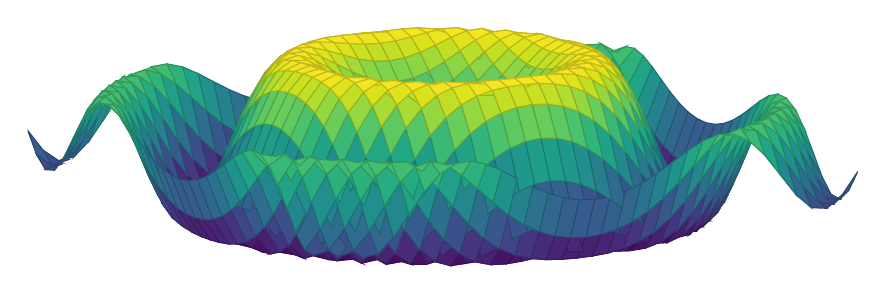
\begin{tikzpicture}
        \begin{axis}[
            colormap/viridis,
            hide axis,
            view={60}{30},
            width=\linewidth,
            height=6cm
        ]
        \addplot3[
            surf,
            samples=35,
            domain=-2.5:2.5,
            y domain=-2.5:2.5,
            z buffer=sort
        ] 
        {sin(deg(x^2 + y^2)) * exp(-0.1*(x^2+y^2))};
        \end{axis}
    \end{tikzpicture}
    \caption{Surface plot of a harmonic scalar field undergoing exponential spatial decay, rendered natively in \LaTeX{}.}\label{fig:wave}
\end{figure}

\section{Conclusion}

The \textit{Equimandots} architecture proves that plain-text editors, when heavily 
augmented with Lua scripting\cite{astronvim} and symbolic backends, provide 
an unparalleled environment for scientific authoring\cite{castel2019}. 

\begin{thebibliography}{9}
\bibitem{castel2019}
G. Castel, \textit{How I'm able to take notes in mathematics lectures using \LaTeX{} and Vim}, castel.dev, 2019.
\bibitem{astronvim}
AstroNvim Community, \textit{AstroNvim: A Neovim IDE}, 2024.
\end{thebibliography}

\end{document}
